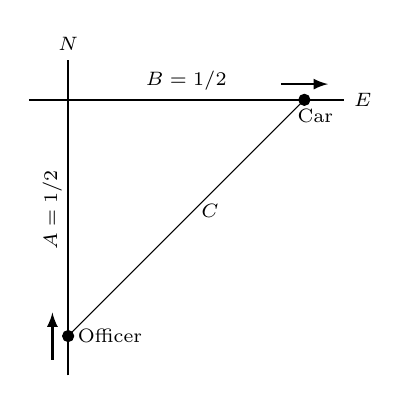
\begin{tikzpicture}[>=latex]

\draw(0,0) -- (3,0) node [pos=.5,above] {\scriptsize $B=1/2$} -- (0,-3) node [pos=.4,below] {\scriptsize $C$}-- (0,0) node [pos=.5,rotate=90,shift={(.1,.2)}] {\scriptsize $A=1/2$};

\draw[thick] (0,-3.5) -- (0,.5) node [above] {\scriptsize $N$};
\draw[thick] (-.5,0) -- (3.5,0) node [right] {\scriptsize $E$};
\filldraw[fill={\colortwo},draw={\colortwo}] (0,-3) circle (2pt) node [right] {\scriptsize Officer};
\filldraw[fill=black,draw=black] (3,0) circle (2pt) node [below ] {\scriptsize \quad Car};

\draw[->,thick] (-.2,-3.3) -- (-.2,-2.7);
\draw[->,thick] (2.7,.2) -- (3.3,.2);

\end{tikzpicture}

